\documentclass{beamer}
\usetheme{Singapore} % My favorite!
\setbeamercovered{invisible}
% To remove the navigation symbols from 
% the bottom of slides%
\setbeamertemplate{navigation symbols}{} 
%
\usepackage{tikz}
\usepackage{pgf}
\usepackage{xxcolor}
\usetikzlibrary{arrows,shadows,petri}
%                              wg. tokens
\usepackage{verbatim}
\usepackage{graphicx}
%\usepackage{bm}         % For typesetting bold math (not \mathbold)
%\logo{\includegraphics[height=0.6cm]{yourlogo.eps}}
%
\title[Short title of the talk]{Network Based Modeling for the Spread of Scientific Ideas }
\author{Mayra Berm\'udez, Sarah Grimm \& Sayed-Rzgar Hosseini}
\institute[U of X]
{ ETH Zurich \\
\medskip
%{\emph{email@domain.ca}}
}
\date{\today}
% \today will show current date. 
% Alternatively, you can specify a date.
%

\listfiles
\begin{document}
%
\begin{frame}
\titlepage
\end{frame}
%
\begin{frame}
\tableofcontents[pausesections]
\end{frame}
%
\section{Spread of scientific ideas}
%
\begin{frame}
{Spread of scientific ideas}
\begin{figure}
[htp]
\begin{center}
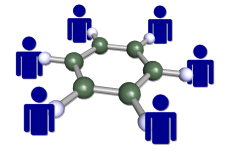
\includegraphics{science_network_150}
\end{center}
\label {fig1}
\end{figure}
\end{frame}
%
\begin{frame}
\alert{In this slide I' would like to add a figure very similar to the last one but with some labels and different color in the nodes. A draft of it is the Figure1beamer. I haven't manage to put here! Hopefully I'll do it later!}
\end{frame}
%
\section{Motivations}
%
\begin{frame}
\frametitle{Introduction and Motivations}
\begin{itemize}
\item But how do ideas spread? \pause
\item Research has shown that not only does the nature of information or innovation influence the diffusion of it, but also that the structure of a network influences the diffusion dynamics. \pause
\end{itemize}
\end{frame}
%
\begin{frame}
\begin{itemize}
\item Here, we try to simulate the spread of scientific ideas in different networks. \pause
\item The model presented is based on two studies: one that investigated critical parameter values for complex contagion and another that investigated critical values of a rewiring parameter.\pause
\end{itemize}
\end{frame}
%
\begin{frame}
{Fundamental Questions}
The main goals of this simulation study are to investigate how network structure influences the distribution of ideas, and how the distribution of ideas influences network structure.
\end{frame}
%
\section{Definitions needed}
\begin{frame}
{Some terminology}
\alert {What other definitions should I put here? Paralell, nonparallel???}
\end{frame}
%
\begin{frame}
\textbf{Neighborhood index:}  The fraction of the holders of the same idea who are neighbor as well averaged over all ideas.\pause \\
\textbf{Intra-idea distance:} The average distance between holders of the same idea in the network.\pause \\
\textbf{Dominant frequency :} The frequency of the dominant idea in the network at each time steps of the simulation.\pause \\
\textbf{Average dominance time:} The average number of time steps in which the dominant idea keeps its dominance.\pause \\
\textbf{Novelty index:} The fraction of newly generated ideas.\pause 
\end{frame}
%
\begin{frame}
\textbf{Average shortest path :} The average number of steps along the shortest paths for all possible pairs of network nodes.\pause \\
\textbf{Clustering coefficient:} A measure of degree to which nodes in a graph tend to cluster together.\pause \\
\textbf{Degree of connectivity :} The number of edges incident to the vertex.\pause \\
\textbf{Connected component:} A subgraph in which any two vertices are connected to each other by paths, and which is connected to noadditional vertices in the supergraph.\pause \\
\textbf {Diameter of network:} The longest of all the calculated shortest paths in a network.

\end{frame}
%
\section{Elements of the model}
%
\begin{frame}
{During the study we vary:} 
\textbf{Parameters}
\begin{itemize}
\item Probability of rewiring $\phi$
\item Rate of innovation $\alpha$
\item Complex contagion threshold  $\delta$ respectively) 
\end{itemize} \pause
\textbf{Network structures}
\begin{itemize}
\item Random
\item Scale free
\item Small world
\item Caveman
\end{itemize}\pause
\textbf{Idea distributions}
\begin{itemize}
\item Random
\item Parallel
\item Nonparallel
\end{itemize}
\end{frame}
%
\begin{frame}
{Parameters}
\textbf{$\phi$:} Is a value from zero to one, and is the probability that one of the edges of a randomly chosen node \emph{i} will be changed to connect to another node \emph{j} that \emph{i} is unconnected with.\\ \pause
\textbf{$\alpha$:} Is the probability that at each time step a node may `come up with a new idea' .\\ \pause
\textbf{$\delta$:} The node threshold  to the general model in order to investigate the behaviour of \textbf{complex contagion.}
\end{frame}
%
\begin{frame}
{What is complex contagion?}
We included this element motivated by a study by \alert{citet*{CM2007}}. \\ \pause
Simple contagion well suited for modeling the spread of diseases \\ \pause
But is enough to hear about a new scientific idea for the first time to adopt it? \\ \pause
$\Rightarrow$ Complex contagion \\\pause
How to implement it in the model?\pause
\begin{itemize}
\item It is either a fixed number (greater than one)\pause
\item \textbf{It is a fraction}
\end{itemize}

\end{frame}
%
\begin{frame}
{Network structures}
\alert{I'll include here some images to illustrate them}
\end{frame}
%
\begin{frame}
{Idea distributions}
\alert{also images with cave man model}
\end{frame}
%
\section{Model}
%
\begin{frame}
\frametitle{Description of the Model}

The model used here is based on a study by \alert{citet*{HN2006}}. \\
Each simulation begins with a specified network structure as well as a distribution of the `idea' (or state) of the nodes.\\ \pause
At each time step a node selected at random either: \pause
\begin{itemize}
\item Changes its idea to that of one of its neighbours' ideas if its frequency surpasses a defined threshold\pause
\item Rewires to connect with a node that has the same idea\pause or
\item Generates a novel idea (this is the innovation parameter). 
\end{itemize}
\end{frame}
%
\section{Questions}
\begin{frame}
{Effects of Network Structure on Idea Distribution}
\begin{itemize}
\item Given a starting network and a random idea distribution, how do different network structures (see Section ) affect the distance between nodes that have the same idea (intra-idea distance)? \pause
\item How do they affect the neighbourhood index? \pause
\item How do they change the emergence of dominant ideas and their time of dominance? How do their effects depend on the values of $\phi$, $\alpha$ and $\delta$?\pause
\end{itemize}
\end{frame}
%
\begin{frame}
{Effects of Idea Distribution on Network Structure}
\begin{itemize}
\item Given a starting idea distribution and a caveman network structure, how do different idea distributions affect the average path length and diameter of the network? \pause
\item Do they change the number of connected components in the network?\pause
\item Do clusters form differently, and how does the clustering coefficient change? \pause
\item What does the distribution of node degree looks like? \pause
\item How do these effects depend on the values of $\phi$, $\alpha$, and $\delta$?\pause
\end{itemize}
\alert{should we mention something about the initial idea distribution in phase 2?? (parallel, nonparallel, random)}
\end{frame}

\section{Simulation}
\begin{frame}
\frametitle{Implementation}
\textbf{Phase 1:} Corresponding to the study  of the effect of network structure on the idea distribution.\\ \pause
\textbf{Phase 2:} Where we study how the distribution of the ideas affect the topology of the network. \\ \pause
\end{frame}
%
\begin{frame}
\noindent \textbf{Step 1:} Network structure is chosen and we generate the adjacency matrix corresponding to that structure. The initial idea distribution is also generated.\\ \pause
\textbf{Step 2:} The updating process is done onto the chosen network structure.\\ \pause
\textbf{Step 3:} At this step a series of functions are called to get the results.
\end{frame}
%
\section{Results}
%
\begin{frame}
\alert{We have too many results and I don't think that we have time enough to mention everything, what du you think? In case you think the same, which ones do you think are the most interestings?}
\end{frame}
%
\begin{frame}
\frametitle{Summary and Outlook}
{Conclusions}
\begin{itemize}
\item Our results support the general idea that network structure and qualities of the ideas held in them may mutually influence each other. \pause
\item The more rigid the structure of a network was, the more likely that the intra-idea distance and neighbourhood index of the network was larger.\pause
\item A network in which the pattern of ideas held by the nodes are `in accord' within the clusters of the caveman network maintained more of the structure features of a caveman network. \pause 
\item Networks with a random pattern of ideas or with a pattern with more `disaccord' within the clusters resulted in a structure that began to resemble a random graph more than a caveman network\pause
\end{itemize}
\end{frame}
%
\begin{frame}
Thus, in addition to the structure of networks and the pattern of ideas in them, complex contagion thresholds, innovation rates, and the probability of creating new connections (while reflecting `preferences' of being connected with like-minded others) tend to influence features of the network. 
\end{frame}
%
\begin{frame}
{Further ??}
Several extensions to the proposed model could be investigated to better understand the relationships between network structure and idea distribution.\\ \pause

\begin{itemize}
\item Rewiring criteria\pause
\item Complex contagion and innovation \pause
\item Random idea adoption
\end{itemize}
\end{frame}
%






\end{document}